\begin{tiny}(Ecr01)\end{tiny}
Pour les courbes suivantes, {\'e}tudier les points demand{\'e}s et reconnaitre le support parmi les figures proposées\\
% use packages: array
\renewcommand{\arraystretch}{3.6}
\begin{tabular}{|c|p{3.1cm}|p{3.8cm}|}\hline 
1 & $(\frac{2t}{t^{2}-1},\frac{(t+1)^{2}}{t^{2}})$ & points doubles, branches infinies. \\ \hline 
2 & $(\cos 3t,\sin 2t)$ & points multiples. \\ \hline
3 & $(t+\frac{1}{t},t^{2}+\frac{1}{t^{2}})$ & {\'e}quation cart{\'e}sienne. \\ \hline
4 & $(\frac{t^{3}}{(t-1)(t+2)},\frac{t(t-2)}{t-1})$ & branches infinies. \\ \hline
5 & $(te^{t},\frac{1}{t}e^{t})$ & branches infinies, points d'inflexion. \\ \hline
6 & $(t(1-e^{t}),\ln (\cosh t))$ & branches infinies, points stationnaires. \\ \hline
7 & $\begin{aligned}
(\frac{1}{t}+\frac{2}{t+1}+\frac{3}{t-1},\\
\frac{2}{t}+\frac{3}{t+1}+\frac{1}{t-1})  
 \end{aligned}$
 & branches infinies. \\ \hline
\end{tabular}
\begin{figure}[ht]
   \centering
   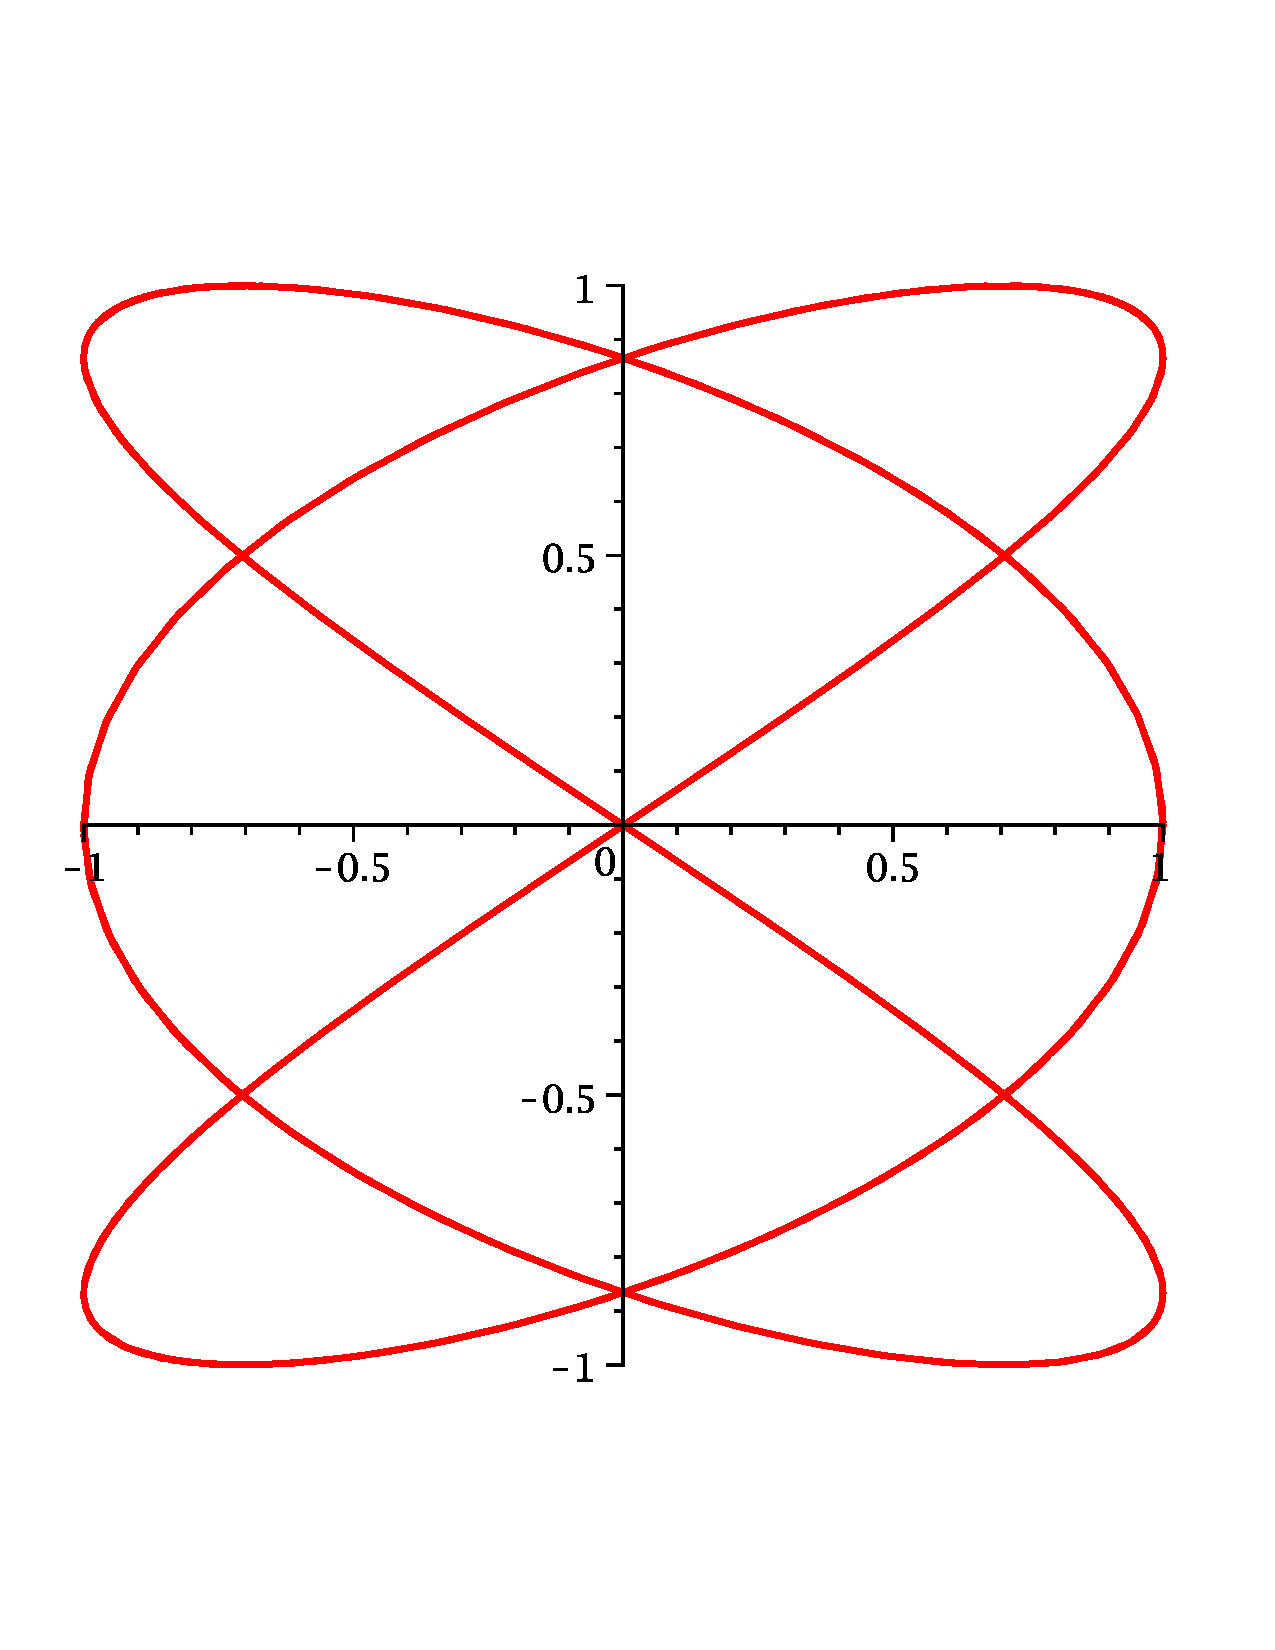
\includegraphics[width=5cm]{Ecr01_1.pdf}
   \caption{Exercice \arabic{enumi} : courbe 1}
\end{figure}
\begin{figure}[ht]
   \centering
   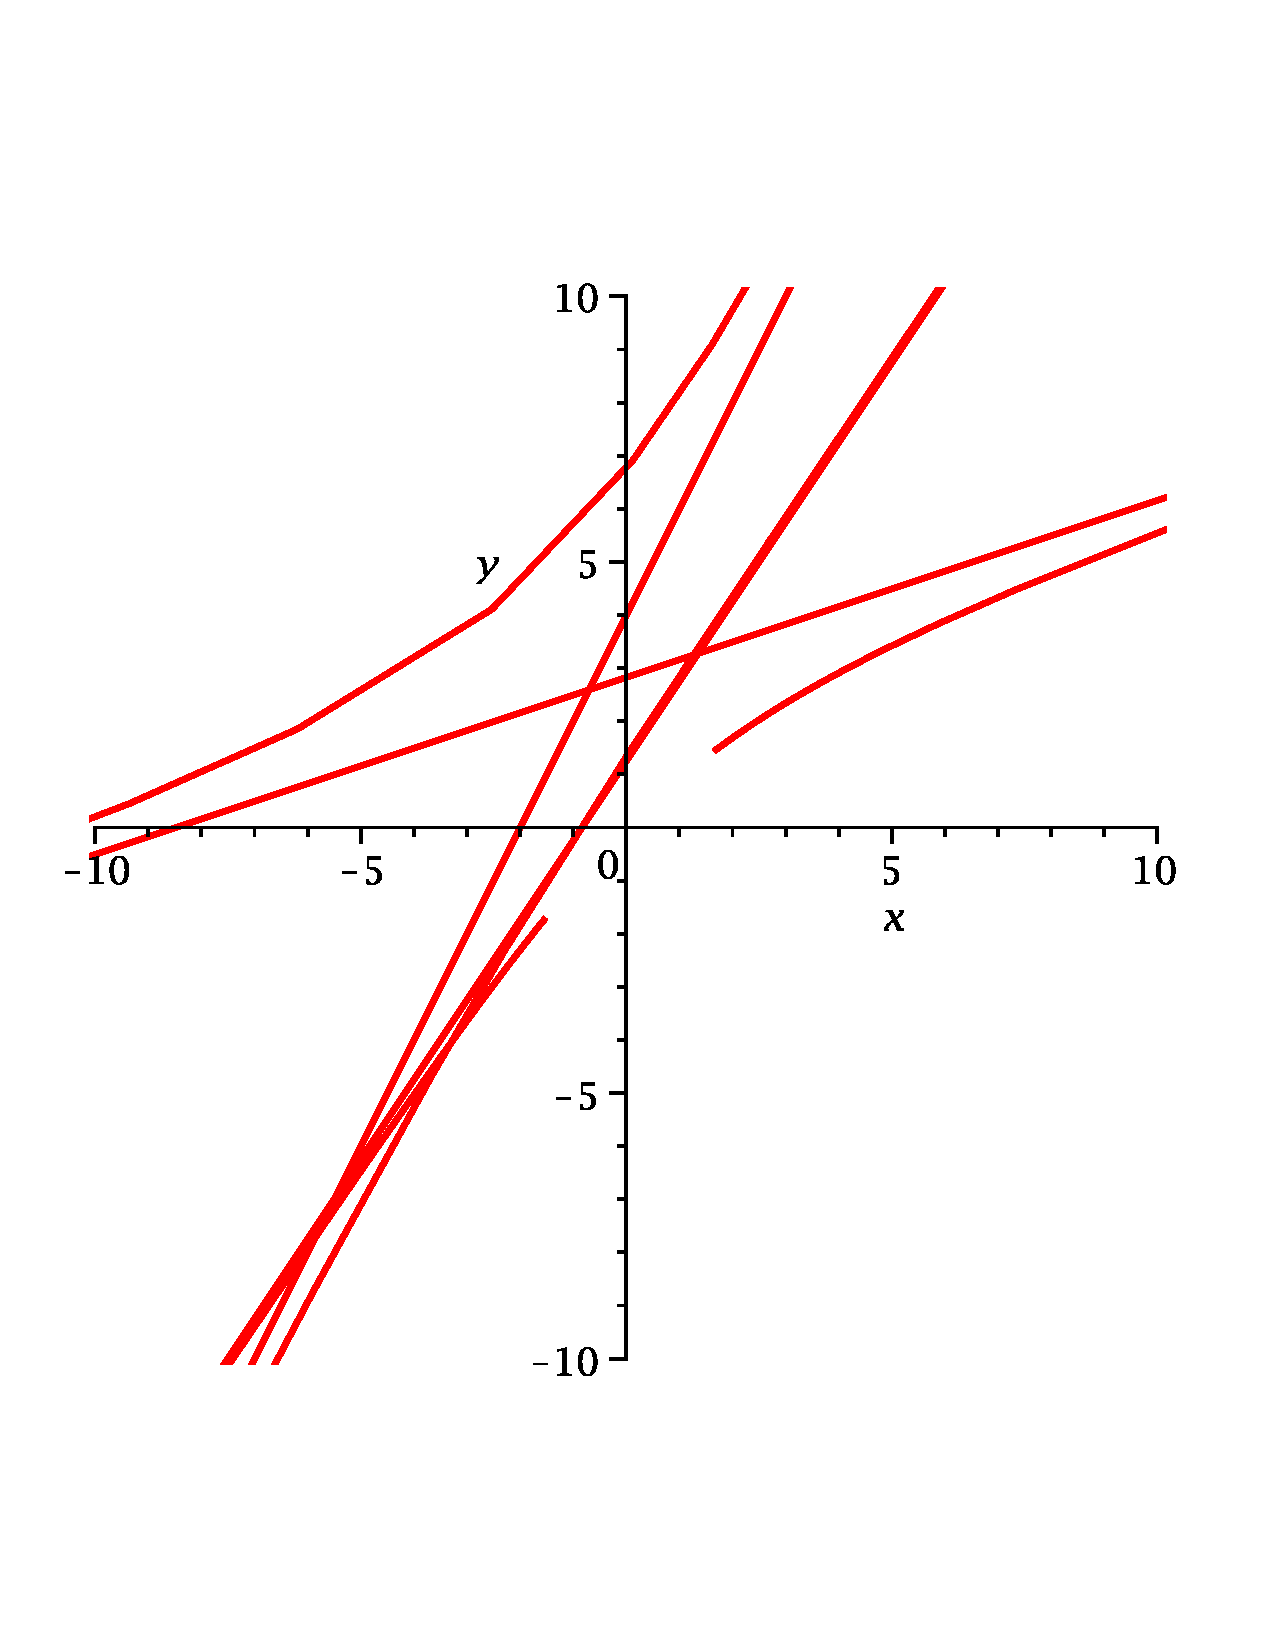
\includegraphics[width=5cm]{Ecr01_2.pdf}
   \caption{Exercice \arabic{enumi} : courbe 2}
\end{figure}
\begin{figure}[ht]
   \centering
   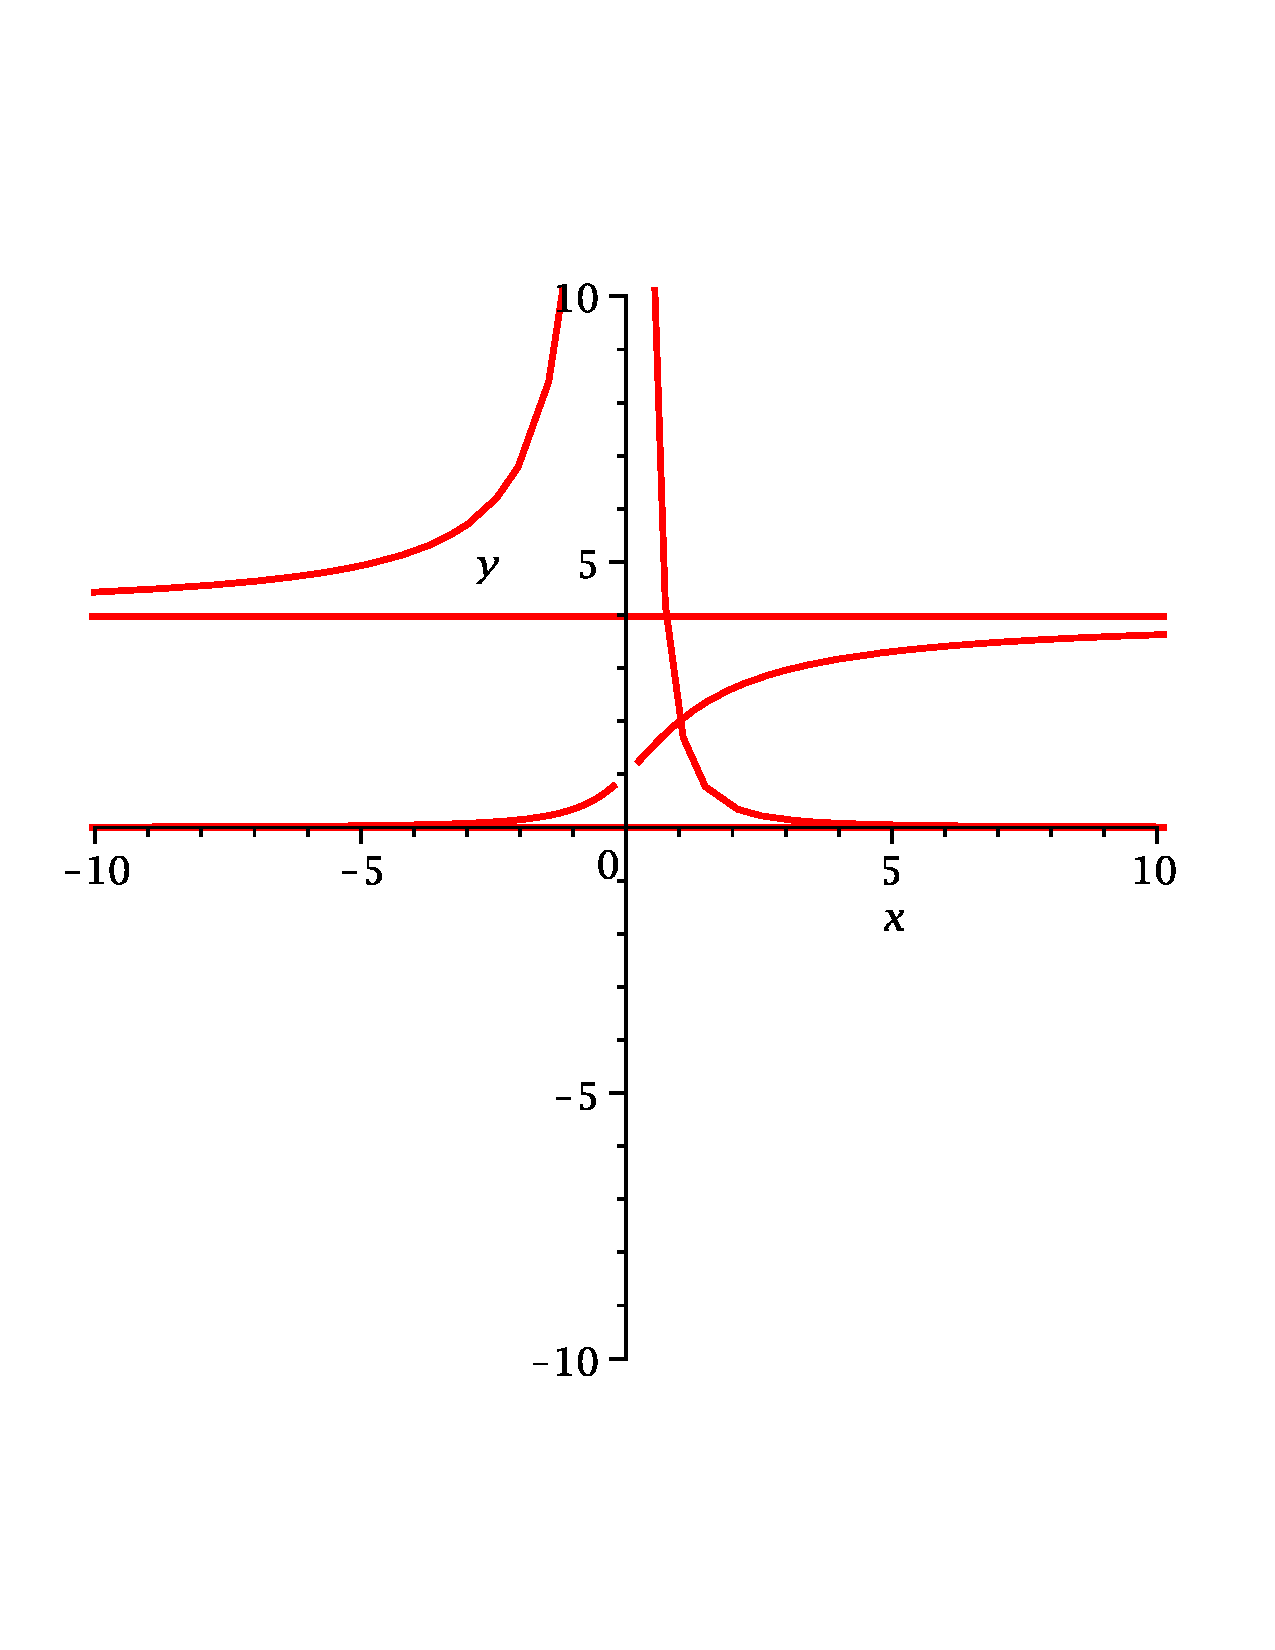
\includegraphics[scale=0.25]{Ecr01_3.pdf}
   \caption{Exercice \arabic{enumi} : courbe 3}
\end{figure}
\begin{figure}[ht]
   \centering
   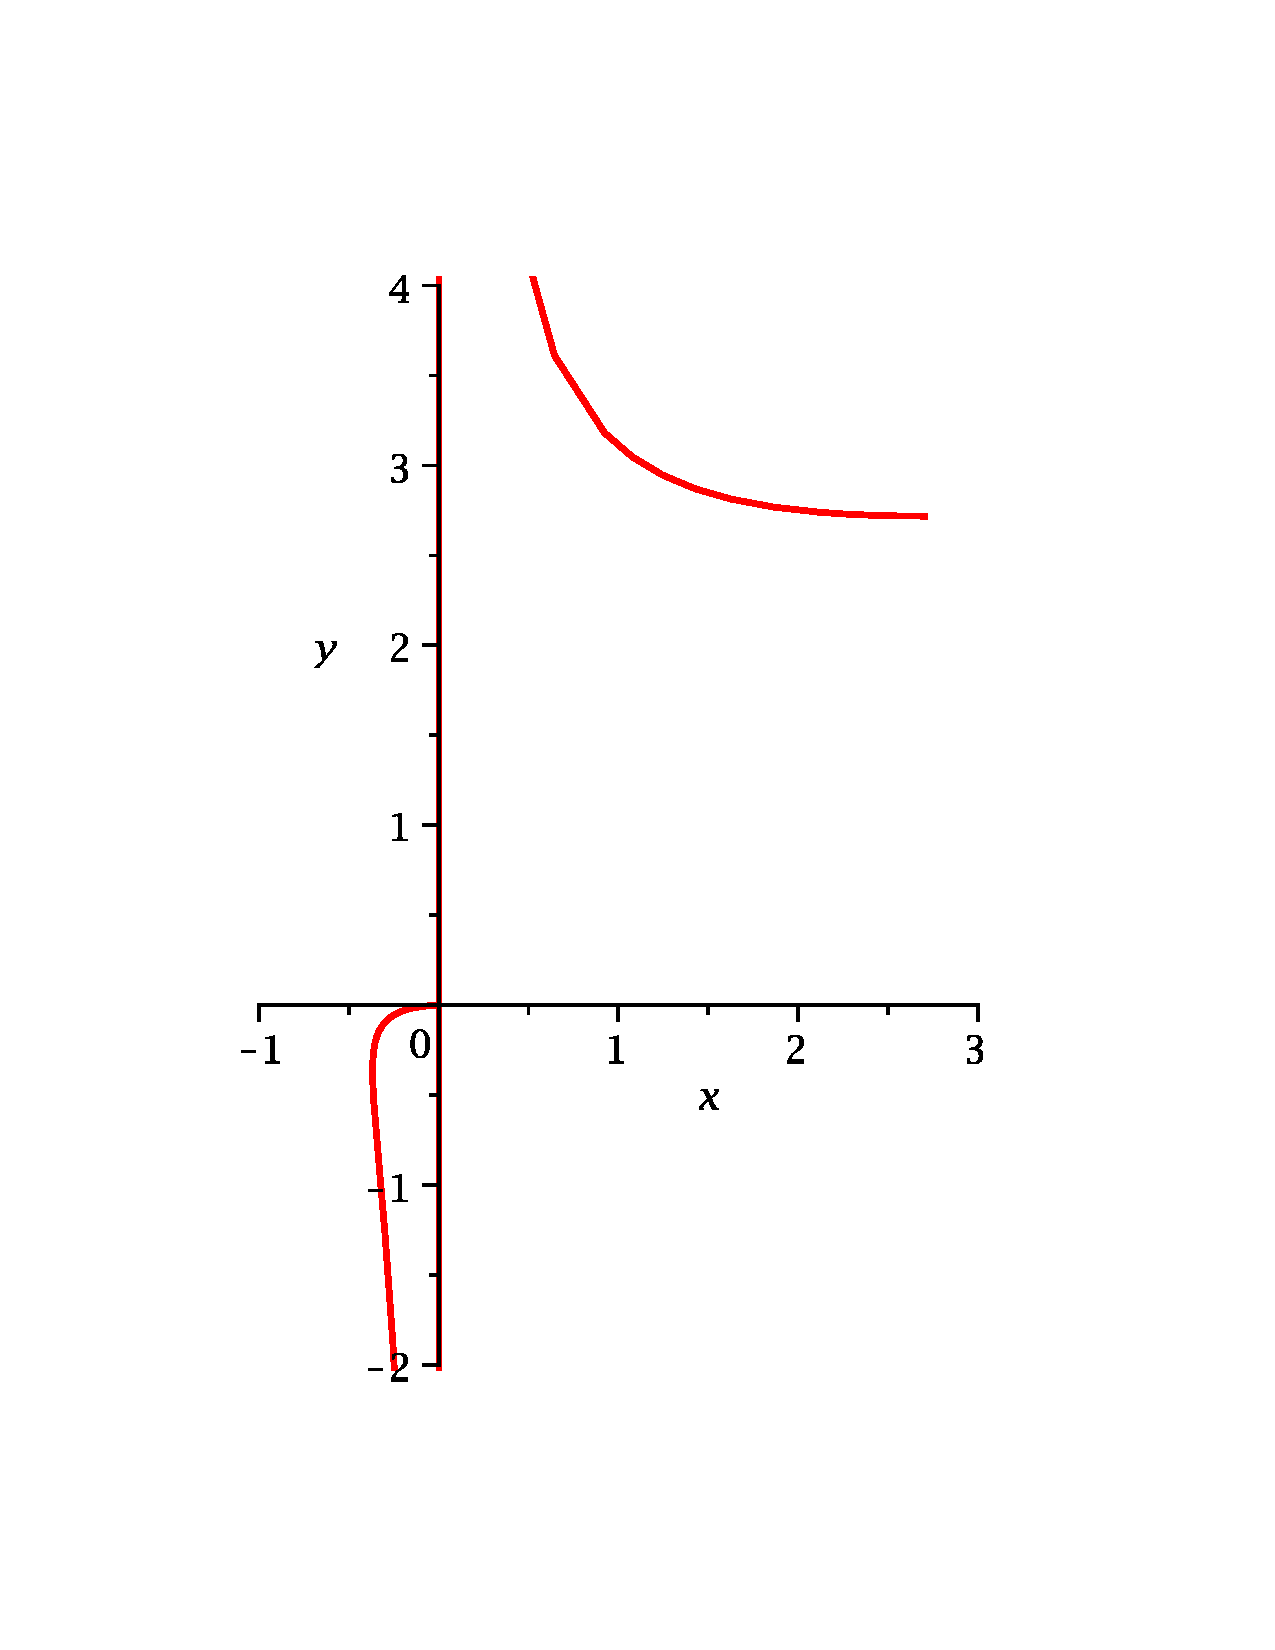
\includegraphics[scale=0.25]{Ecr01_4.pdf}
   \caption{Exercice \arabic{enumi} : courbe 4}
\end{figure}
\begin{figure}[ht]
   \centering
   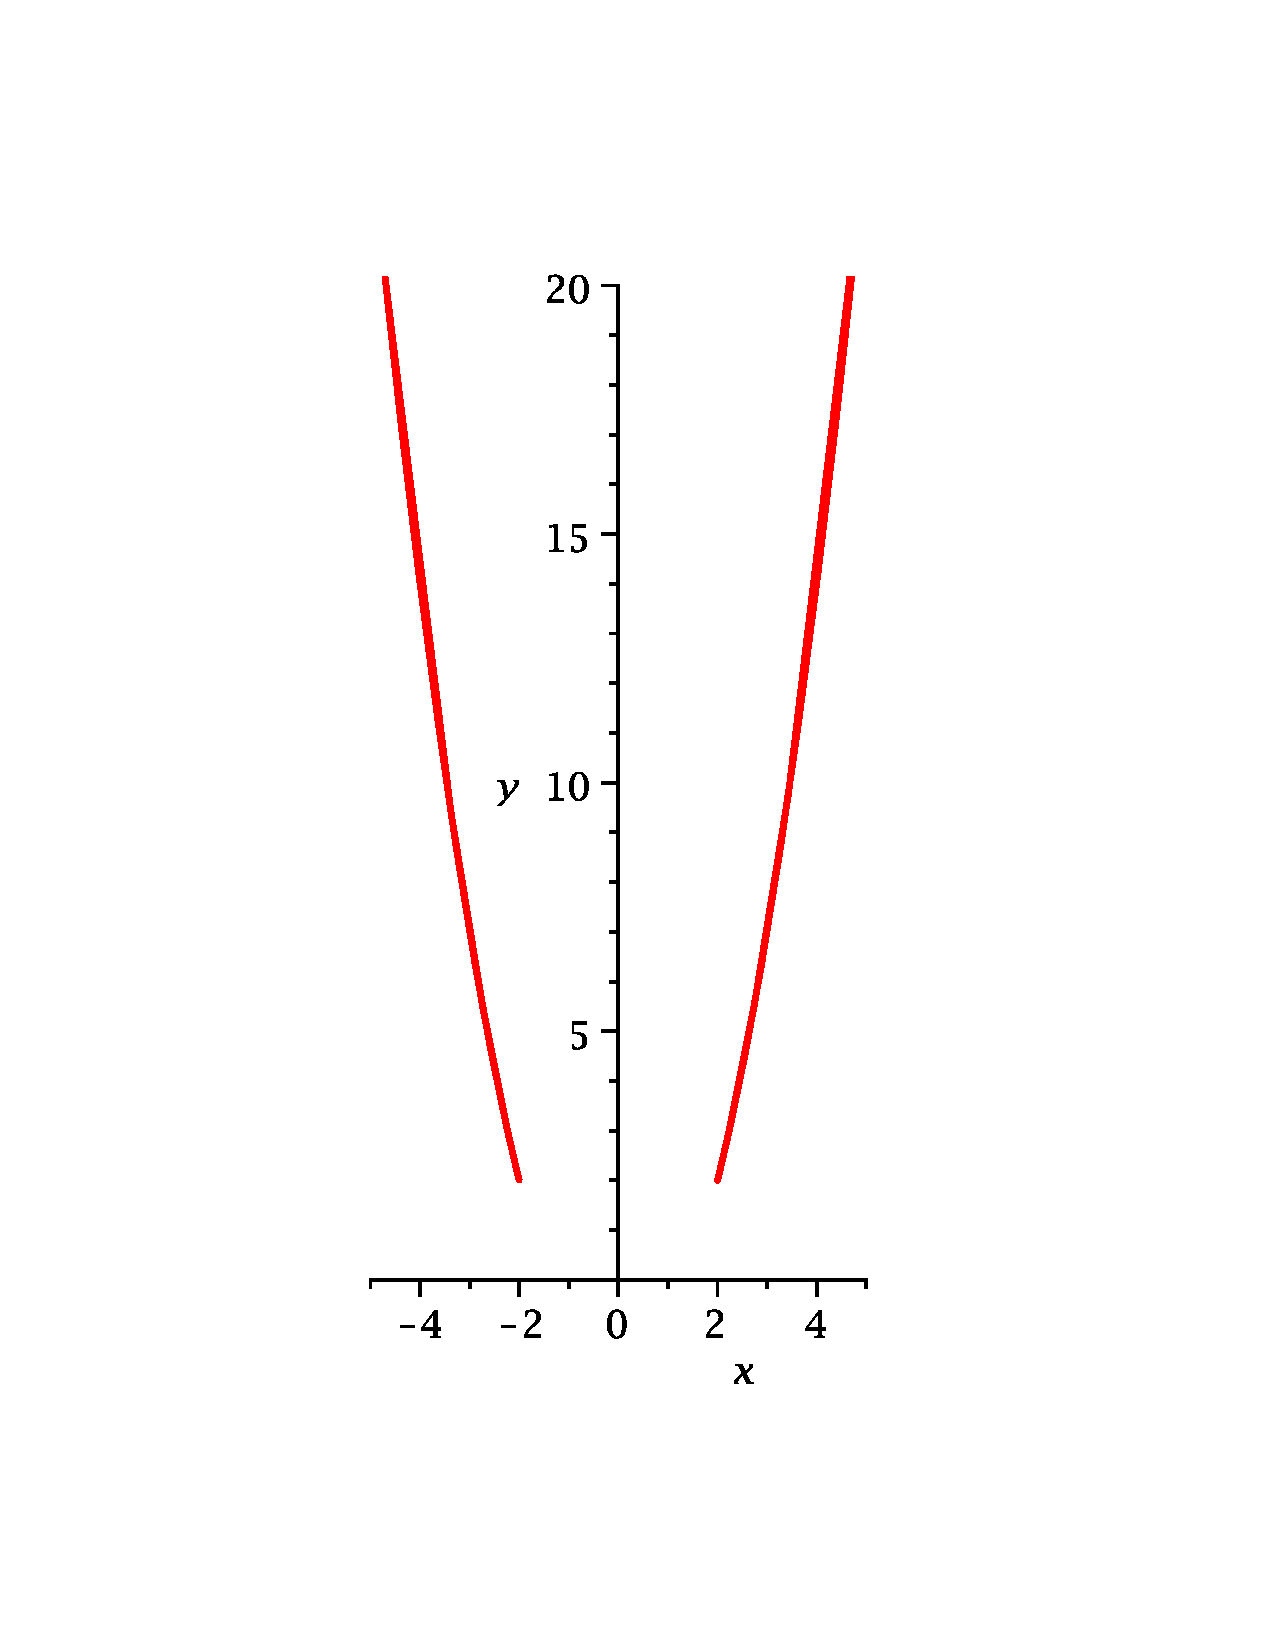
\includegraphics[scale=0.25]{Ecr01_5.pdf}
   \caption{Exercice \arabic{enumi} : courbe 5}
\end{figure}
\begin{figure}[ht]
   \centering
   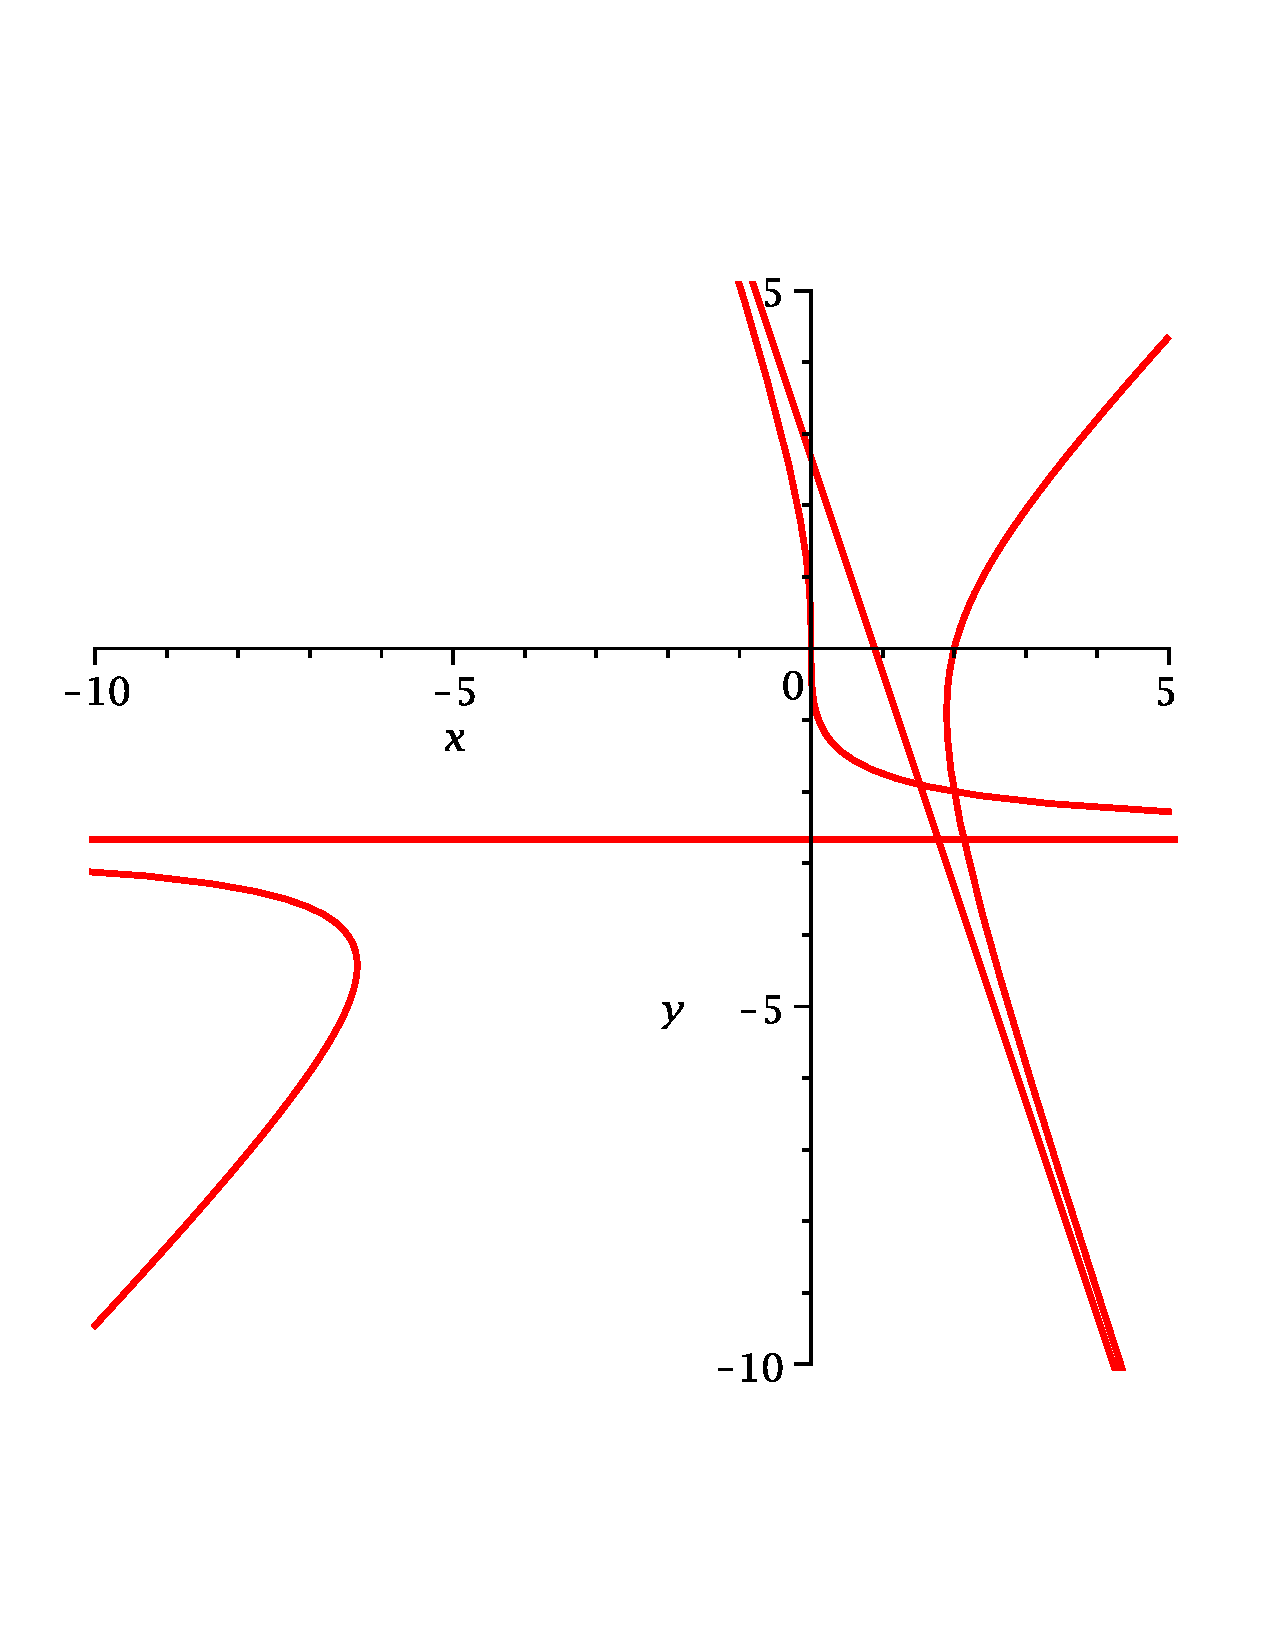
\includegraphics[scale=0.25]{Ecr01_6.pdf}
   \caption{Exercice \arabic{enumi} : courbe 6}
\end{figure}
\begin{figure}[ht]
   \centering
   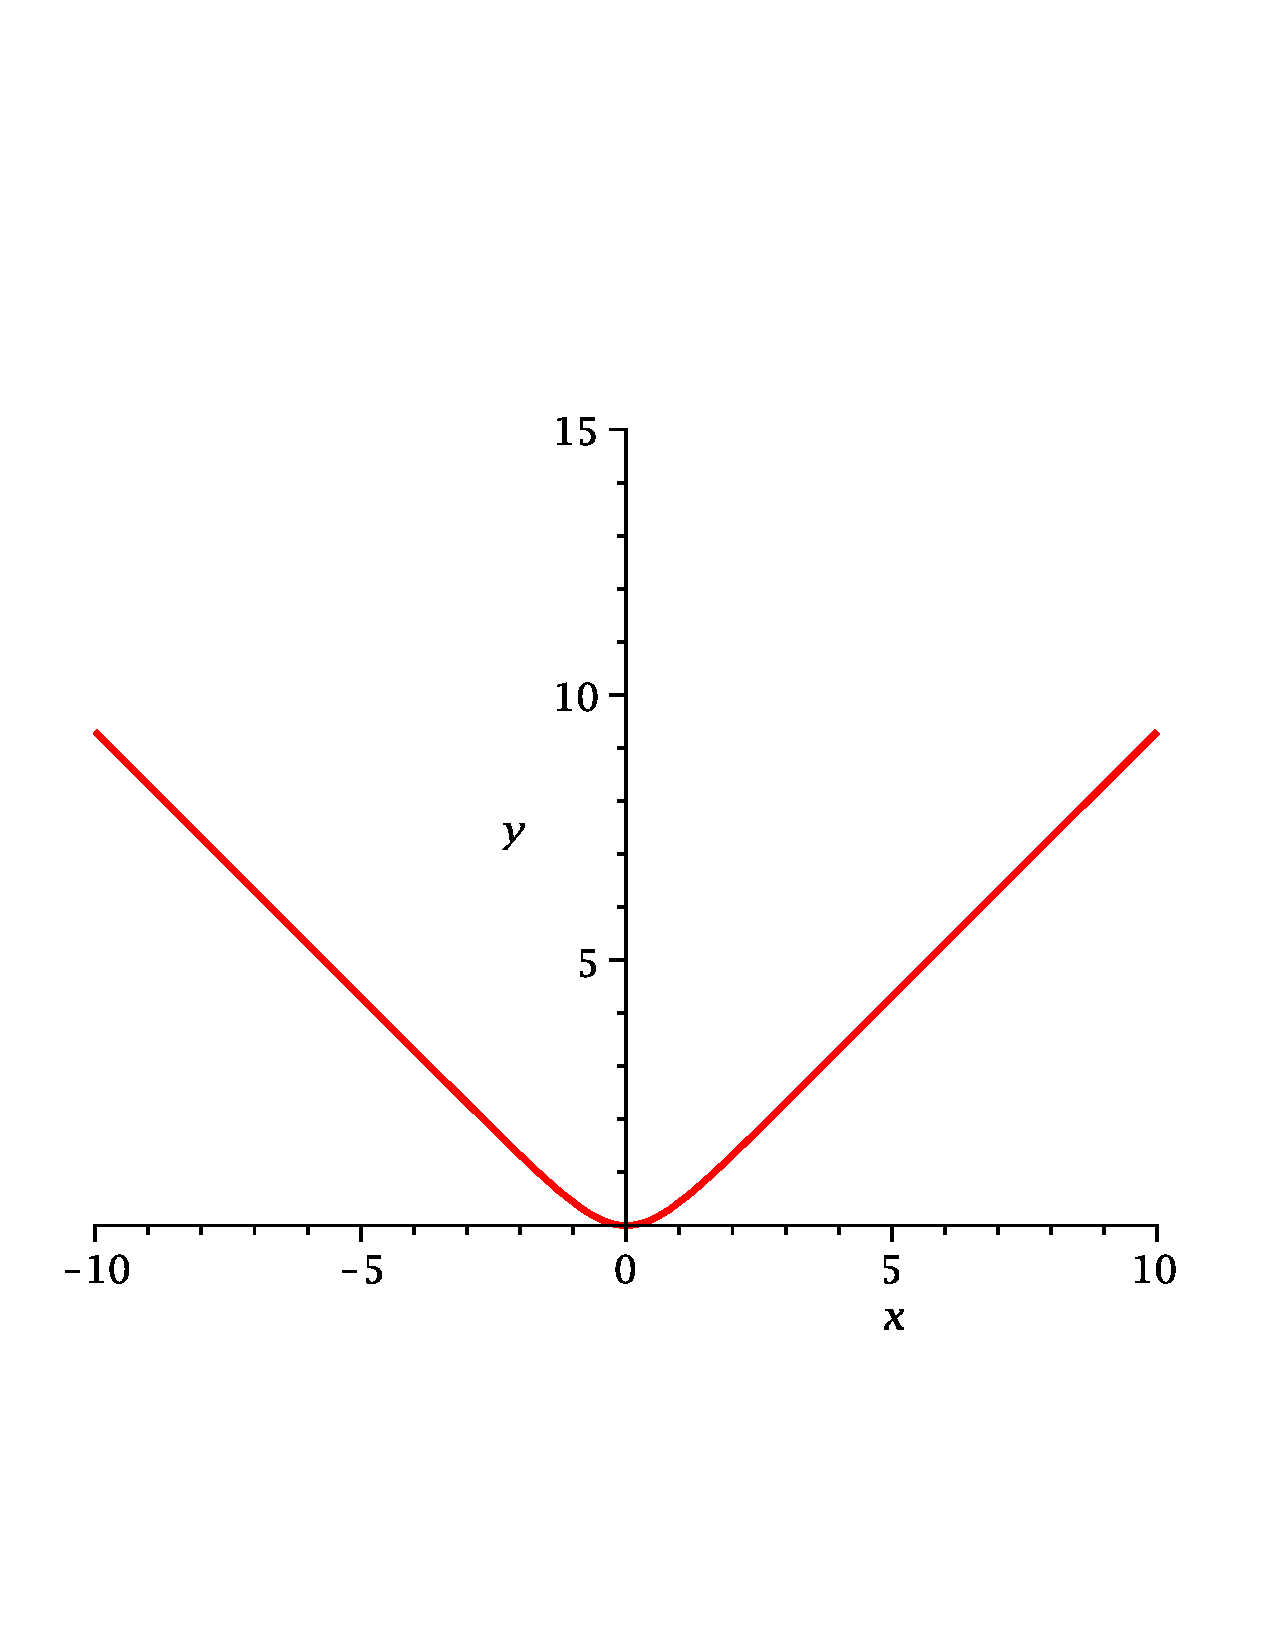
\includegraphics[scale=0.25]{Ecr01_7.pdf}
   \caption{Exercice \arabic{enumi} : courbe 7}
\end{figure}
Pour la recherche des points multiples de la deuxième ligne du tableau, on pourra montrer que si $t_1$ et $t_2$ sont les paramètres d'un (vrai) point multiple alors ils sont tous les deux congrus à $0$ ou a $\frac{\pi}{4}$ modulo $\frac{\pi}{6}$. Pour déterminer les points multiples former les tableaux des coordonnées pour ces valeurs du paramètre et chercher les doublons.  
